%----------------------------------------------------------------------------------------
%	PAGE 3
%----------------------------------------------------------------------------------------
\section{Introduction}
\begin{frame}
\sectionpage
%\begin{center}
%\Large\bf{Methodolody}
%\end{center}
\end{frame}

%----------------------------------------------------------------------------------------
%	PAGE 4
%----------------------------------------------------------------------------------------
\begin{frame}
\frametitle{Background}
In high-dimensional statistics, much work has been made on consistency for prediction, estimation of high-dimensional objects or variable selection.
\begin{itemize}
\item[$\blacksquare$] Regularized linear regression
  \begin{itemize}
  \item[$\blacktriangleright$] $\ell_{1}$ regularized methods
  \item[$\blacktriangleright$] non-convex penalized methods
  \item[$\blacktriangleright$] Greedy methods
  \item[$\blacktriangleright$] screening methods
  \ldots
  \end{itemize}
\end{itemize}
\end{frame}

%----------------------------------------------------------------------------------------
%	PAGE 5
%----------------------------------------------------------------------------------------
\begin{frame}
\frametitle{Background}
Among last decades, few work has been done for constructing confidence intervals or doing statistical testing in high-dimensional testing sparse models.
\begin{itemize}
\item[$\blacksquare$] Existing variable selection approaches based on selection consistency theory typically requires a uniform signal strength condition:
    \begin{equation}
    \label{ussc}
    \hbox{$\min_{\beta_j\neq 0}$} |\beta_j| \ge C\sigma\sqrt{(2/n)\log p},\ C>1/2,
    \end{equation}

\item[$\blacksquare$] when weak signal exists, consistent estimation of the distribution
of the least squares estimator after model selection is impossible.(Leeb and Potscher,2006)

\item[$\blacksquare$] Conservative statistical inference after model selection or classification may not yield sufficiently accurate confidence regions or p-values when number of variables is large.(Berk et.al 2010; Laber and Murphy 2011).
\end{itemize}
\end{frame}

%----------------------------------------------------------------------------------------
%	PAGE 6
%----------------------------------------------------------------------------------------
\begin{frame}
\frametitle{Proposed method}
\begin{itemize}
\item[$\blacksquare$] Low dimensional projection(LDP) approach has significance:
  \begin{enumerate}[(1)]
  \item Construct confidence intervals for regression coefficients
  \item Without requirement of the uniform signal strength condition
  \end{enumerate}
\end{itemize}
\end{frame}

%----------------------------------------------------------------------------------------
%	PAGE 7
%----------------------------------------------------------------------------------------
\section{Methodology}
\begin{frame}
\sectionpage

\end{frame}


%----------------------------------------------------------------------------------------
%	PAGE 8
%----------------------------------------------------------------------------------------
\begin{frame}
\frametitle{Model setting}

\begin{itemize}

\item[$\blacksquare$] Constructing confidence intervals for the individual regression coefficients and their linear combination in the linear model,% (unobservable), %the response vector
\begin{equation}
\label{LM}
\by = {\bX}\bbeta + \varepsilon, \qquad \mathbf{\varepsilon} \sim \mathcal{N}(\bzero,\sigma^2\bI)
\end{equation}
where $\by \in \mathbb{R}^{n}$ is a response vector, $\bX=(\bx_{1},\ldots,\bx_{p})\in \mathbb{R}^{n\times p}$ is a design matrix with columns $\bx_{j}$ and $\bbeta=(\beta_{1}, \ldots, \bbeta_{p}) \t $ is a vector of unknown regression coefficients.
%$X\in {{\mathbb{R}}^{n\times p}}$

\vspace{3mm}

\begin{itemize}
      \item[-]  Standardize the design to $\|\bx_{j}\|^{2}_{2}=n$.

      \medskip

      \item[-] The design matrix $\bX$ is assumed to be deterministic.

\end{itemize}

\end{itemize}


\end{frame}


%----------------------------------------------------------------------------------------
%	PAGE 9
%----------------------------------------------------------------------------------------
\begin{frame}
\frametitle{Least squares estimator}
\begin{itemize}

\item[$\blacksquare$] In classical theory of linear models, the least squares estimator of an estimable regression coefficient $\bbeta_{j}$ can be written as  % (unobservable), %the response vector
\begin{equation}
\hat{\bbeta}^{(lse)}_{j} := (\bx^{\bot}_{j})\t \by /(\bx^{\bot}_{j})\t \bx_{j},
\end{equation}
where $\bx^{\bot}_{j}$ is a projection of $\bx_{j}$ to the orthogonal complement of column space of $\bX_{-j}=(\bx_{k},k\neq j)$.

\item[$\blacksquare$] The $\bx^{\perp}_{j}$ is defined by
\begin{itemize}
      \item[-] $(\bx^{\bot}_{j})\t \bx_{k}=\bzero $, for $ \forall k\neq j$.
      \medskip
      \item[-] $(\bx^{\bot}_{j})\t \bx_{j}=\|\bx_{j}\|^{2}_{2}$.

\vspace{3mm}

\end{itemize}

\end{itemize}


\end{frame}


%----------------------------------------------------------------------------------------
%	PAGE 10
%----------------------------------------------------------------------------------------
\begin{frame}
\frametitle{Problems}
\begin{itemize}

\item[$\blacksquare$] In high dimensional situation $p>n$, $rank(\bX_{-j})=n$ for all $j$. % (unobservable), %the response vector
\begin{itemize}
\item[$\blacktriangleright$] $\bx^{\bot}_{j}=\bzero$.
\item[$\blacktriangleright$] $\hat{\bbeta}^{(lse)}_{j}$ is undefined.
\end{itemize}
\item[$\blacksquare$] We want to preserve the properties of the least squares estimator.
\begin{itemize}
\item[$\blacktriangleright$] The covariance structure of the least squares estimator:
\end{itemize}
\begin{equation}
\cov(\hat{\bbeta}^{(lse)}_{j},\hat{\bbeta}^{(lse)}_{k})=\sigma^{2} \frac{(\bx^{\bot}_{j})\t \bx^{\bot}_{k}}{\|\bx_{j}\|^{2}_{2}\|\bx_{k}\|^{2}_{2}}
\end{equation}
\item[$\blacksquare$] Motivation of LDPE:
\begin{itemize}
      \item[$\blacktriangleright$] Replace $\bx^{\bot}_{j}$ with $\bz_{j}$.
      \medskip
      \item[$\blacktriangleright$] Relaxing the constraint $\bz_{j}\t \bx_{k}=\bzero$ for $k\neq j$.
\vspace{3mm}

\end{itemize}

\end{itemize}


\end{frame}

%----------------------------------------------------------------------------------------
%	PAGE 11
%----------------------------------------------------------------------------------------
\begin{frame}
\frametitle{Bias-corrected linear estimators}
\begin{itemize}

\item[$\blacksquare$] For any $\bz_{j}$ that is not orthogonal to $\bx_{j}$, the corresponding univariate linear regression estimator satisfies
\begin{equation*}
\hat{\bbeta}^{(lin)}_{j}= \frac{\bz^{T}_{j} \by}{\bz^{T}_{j} \bx_{j}}= \beta_j + \frac{\bz_j^T \varepsilon}{\bz_j^T\bx_j}
+ \sum_{k\neq j}\frac{\bz_j^T\bx_k\beta_k}{\bz_j^T\bx_j}.
\end{equation*}
  \begin{itemize}
  \item[$\blacktriangleright$] Here,  $\hat{\bbeta}^{(lin)}_{j}$ has the same covariance structure with $\hat{\bbeta}^{(lse)}_{j}$.
  \end{itemize}
\item[$\blacksquare$] Note that the bias of $\hat{\bbeta}^{(lin)}_{j}$ is unbounded. It is impossible to have $\bz_{j}\t \bx_{k}=\bzero$ for all $k\neq j \quad (\bz_{j}\neq\bzero)$.
\end{itemize}
\end{frame}


%----------------------------------------------------------------------------------------
%	PAGE 12
%----------------------------------------------------------------------------------------
\begin{frame}
\frametitle{Low dimensional projection estimator}
\begin{itemize}

\item[$\blacksquare$] Bias correction with a non-linear initial estimator $\hat{\bbeta}^{(init)}$:
\begin{equation}
\label{LDPE}
\hat{\bbeta}_{j}=\hat{\bbeta}^{(lin)}_{j} - \sum_{k \neq j}\frac{\bz_{j}\t \bx_{k} \hat{\bbeta}^{(init)}_{k} }{\bz^{T}_{j} \bx_{j}}
=\frac{\bz^{T}_{j} \by}{\bz^{T}_{j} \bx_{j}} - \sum_{k \neq j}\frac{\bz_{j}\t \bx_{k} \hat{\bbeta}^{(init)}_{k} }{\bz^{T}_{j} \bx_{j}}.
\end{equation}
   \begin{itemize}
   %\item[$\blacktriangleright$] One-step self-bias correction from $\hat{\bbeta}^{(init)}$:
   %\medskip
   \item[$\blacktriangleright$] The estimation error of $\hat{\bbeta}_{j}$:
   \begin{equation}
   \label{bias(5)}
   \hat{\bbeta}_{j}-\bbeta_{j}=\frac{\bz^{T}_{j} \varepsilon}{\bz^{T}_{j} \bx_{j}} + \frac{\sum_{k \neq j} \bz_{j}\t \bx_{k} (\bbeta_{k} - \hat{\bbeta}^{(init)}_{k}) }{\bz^{T}_{j} \bx_{j}} \triangleq \bA + \bB.
   \end{equation}
   \item[$\blacktriangleright$] It can be viewed as a sum of noise term and bias term.
   %\vspace{3mm}
   \end{itemize}

\end{itemize}


\end{frame}


%----------------------------------------------------------------------------------------
%	PAGE 13
%----------------------------------------------------------------------------------------
\begin{frame}
\frametitle{Error analysis of LDPE$(1)$}
\begin{itemize}

\item[$\blacksquare$] The approximation error of the LDPE (Term $\bB$) can be controlled:
\begin{equation}
\Big|\sum_{k\neq j}\bz_j^T\bx_k(\beta_k-\hbeta_k^{(init)})\Big|
\le \Big(\max_{k\neq j}\big|\bz_j^T\bx_k\big|\Big)\|\hbbeta^{(init)}-\bbeta\|_1.
\end{equation}
\item[$\blacksquare$] For $\bz_{j}$, define
\begin{equation}
\label{defetatau}
\eta_j = \max_{k\neq j}\big|\bz_j^T\bx_k\big|/\|\bz_j\|_2,\qquad \tau_j = \|\bz_j\|_2/|\bz_j^T\bx_j|.
\end{equation}
   \begin{itemize}
   \item[$\blacktriangleright$] Bias factor $\eta_{j}$: $\eta_{j} \|\hat{\bbeta}^{(init)}-\bbeta\|_{1}$ controls the approximation error.
   \item[$\blacktriangleright$] Noise factor $\tau_{j}$: $\tau_{j} \sigma$ is the standard deviation of noise term.
   %\vspace{3mm}
   \end{itemize}

\end{itemize}


\end{frame}


%----------------------------------------------------------------------------------------
%	PAGE 14
%----------------------------------------------------------------------------------------
\begin{frame}
\frametitle{Error analysis of LDPE $(2)$}
\begin{itemize}

\item[$\blacksquare$] Since $\bz_{j} \t \varepsilon \sim N(\bzero, \sigma^{2} \|\bz_{j}\|^{2}_{2})$, equation $(5)$ yields
\begin{equation}
\label{interval}
\eta_{j}\|\hat{\bbeta}^{(init)}-\bbeta\|_{1}/\sigma=o(1)\Rightarrow \tau^{-1}_{j}(\hat{\bbeta}_{j}-\bbeta_{j})\approx N(\bzero,\sigma^{2}).
\end{equation}
\item[$\blacksquare$] Confidence intervals can be constructed by condition (\ref{interval}) and a consistent estimator of $\sigma$.
%\item[$\blacksquare$] Pick a $\bz_{j}$ with a small $\eta_{j}$ for the asymptotic normality and a small $\tau_{j}$ for efficiency of estimation.
\item[$\blacksquare$] Need to solve:
  \begin{itemize}
  \item[$\blacktriangleright$] Choose proper $\bz_{j}$.
  \item[$\blacktriangleright$] Choose $\hat{\bbeta}^{(init)}$.
% \item[$\blacktriangleright$] Estimate $\sigma$.
  \end{itemize}

\end{itemize}
\end{frame}

%----------------------------------------------------------------------------------------
%	PAGE 15
%----------------------------------------------------------------------------------------
\begin{frame}
\frametitle{How can we choose $\bz_{j}$ ?}
\begin{itemize}

\item[$\blacksquare$] Choose $\bz_{j}$ as the residual of lasso.
\small{
\begin{equation}
\label{lasso}
\bz_j = \bx_j - \bX_{-j} \hat{\gamma}_j,\
\hat{\gamma}_j = \argmin_{\bb}\Big\{\frac{\|\bx_j-\bX_{-j}\bb\|_2^2}{2n}+\lambda_j \|\bb\|_1\Big\}.
\end{equation}
}
\item[$\blacksquare$] Karush-Kuhn-Tucker conditions for equation (\ref{lasso}). \\
                      $\Rightarrow \quad |\bx_k^T\bz_j/n|\le\lambda_{j}$ for all $k \neq j$ \\
                      $\Rightarrow \quad \eta_j\le n\lambda_j/\|\bz_j\|_2$.

\end{itemize}


\end{frame}


%----------------------------------------------------------------------------------------
%	PAGE 16
%----------------------------------------------------------------------------------------
\begin{frame}
\frametitle{How can we pick initial estimator of $\bbeta$?}
\begin{itemize}
\item[$\blacksquare$] The scaled lasso is a joint convex minimization method
\begin{equation}
\big\{\hat{\bbeta}^{(init)},\sigma\big\} = \argmin_{\bb,\sigma}
\Big\{\frac{\|\by-\bX\bb\|_2^2}{2\sigma n} + \frac{\sigma}{2}+\lambda_0\|\bb\|_1\Big\}.
\end{equation}
\item[$\blacksquare$] The scaled lasso is biased, an alternative method scaled lasso-LSE can be applied:
\begin{equation}
\{\hat{\bbeta}^{(init)},\sigma\} = \argmin_{\bb,\sigma}
\big\{\frac{\|\by-\bX\bb\|_2^2}{2\sigma max(n-|\hat{S}^{(scl)}|,1)} + \frac{\sigma}{2}\big\}
\end{equation}
where $\hat{S}^{(scl)}$ is the set of non-zero estimated coefficients produce by scaled lasso.
%$\bb_j=\bzero \quad \forall j \not\in \hat{S}^{(scl)}$
\end{itemize}
\end{frame}


%----------------------------------------------------------------------------------------
%	PAGE 17
%----------------------------------------------------------------------------------------
%\begin{frame}
%\frametitle{Precedure of LDPE}
%\begin{figure}[h]
%  \centering
%  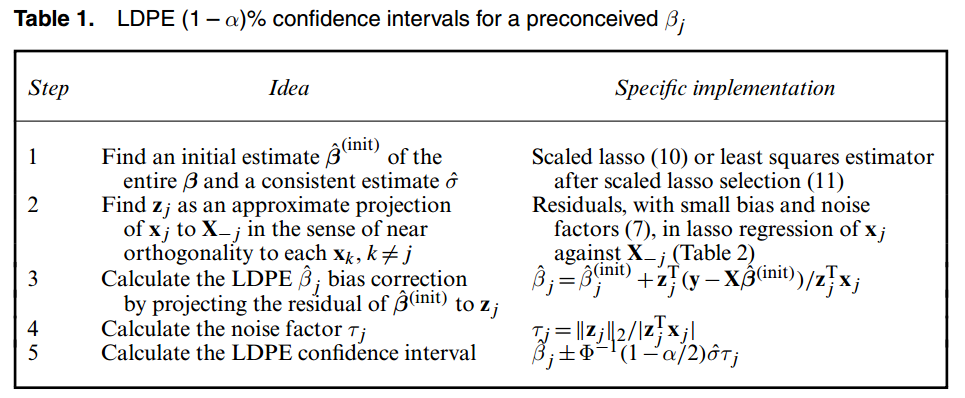
\includegraphics[width=1.0\textwidth]{figs/Table 1.png}
%  \label{Table1}
%\end{figure}
%\end{frame}


%----------------------------------------------------------------------------------------
%	PAGE 17
%----------------------------------------------------------------------------------------
\begin{frame}
\begin{block}{Procedure of computing $\bz_{j}$}
    Along the Lasso path for regressing $\bx_j$ against $\bX_{-j}$, let
%Here is a description of the algorithm.
\begin{equation}
\begin{aligned}
\gamma_j(\lambda) = \arg\min_{\bb} \{\|\bx_j & -\bX_{-j}\bb\|_2^2/(2n) + \lambda\|\bb\|_1\}, \\
\bz_j(\lambda)  & = \bx_j-\bX_{-j}\gamma_j(\lambda), \\
\eta_j(\lambda) = \max_{k\neq j} & |\bx_k^T\bz_j(\lambda)|/\|\bz_j(\lambda)\|_2, \\
\tau_j(\lambda)  = & \|\bz_j(\lambda)\|_2/|\bx_j^T\bz_j(\lambda)|, \\
\end{aligned}
\end{equation}
be the coefficient estimator $\gamma_j$, residual $\bz_j$, the bias factor $\eta_j$, and
the noise factor $\tau_j$, as functions of $\lambda$.
\end{block}
\end{frame}


%----------------------------------------------------------------------------------------
%	PAGE 19  插入代码表格
%----------------------------------------------------------------------------------------
\begin{frame}
  \frametitle{Computation of $\bz_{j}$}
  \scriptsize
  \begin{table}%[ht]
  \caption{Computation of $\bz_j$ from the Lasso (\ref{lasso})}
  \begin{tabular}{cl}
  \toprule
  %\multicolumn{2}{c}{Computation of $\bz_j$ from the Lasso (\ref{Lasso-path-j})}\\
  % for standardized design vectors}\\
  %\midrule
  Input: & an upper bound $\eta_j^*$ for the bias factor, with default value $\eta^*_j=\sqrt{2\log p}$, \\
  & tuning parameters $\kappa_0\in [0,1]$ and $\kappa_1\in (0,1]$; \\
  Step 1: & (verify/adjust $\eta_j^*$ and compute the corresponding noise factor $\tau_j^*$) \\
  & If $\eta_j(\lambda)>\eta_j^*$ for all $\lambda>0$, $\eta_j^* \leftarrow (1+\kappa_1)\inf_{\lambda>0}\eta_j(\lambda)$; \\
  & $\lambda\leftarrow \max\{\lambda: \eta_j(\lambda)\le\eta^*_j\}$,
  $\eta_j^*\leftarrow \eta_j(\lambda)$, $\tau_j^*\leftarrow \tau_j(\lambda)$; \\
  Step 2: & (further reduction of the bias factor)\\
  & $\lambda_j \leftarrow \min\{\lambda: \tau_j(\lambda)\le (1+\kappa_0)\tau^*_j\}$;
  %%%
  \\
  Output: & $\lambda_j$, $\bz_j\leftarrow \bz_j(\lambda_j)$, $\tau_j\leftarrow \tau_j(\lambda_j)$, $\eta_j\leftarrow \eta_j(\lambda_j)$\\
  \bottomrule
  \addlinespace
  \end{tabular}
  \label{table:alg}
  
  \end{table}
  
  \end{frame}


%----------------------------------------------------------------------------------------
%	PAGE 18  插入图片 去掉名字
%----------------------------------------------------------------------------------------
\begin{frame}
\frametitle{Computation of $\bz_{j}$}
\begin{figure}[h]
  \centering
  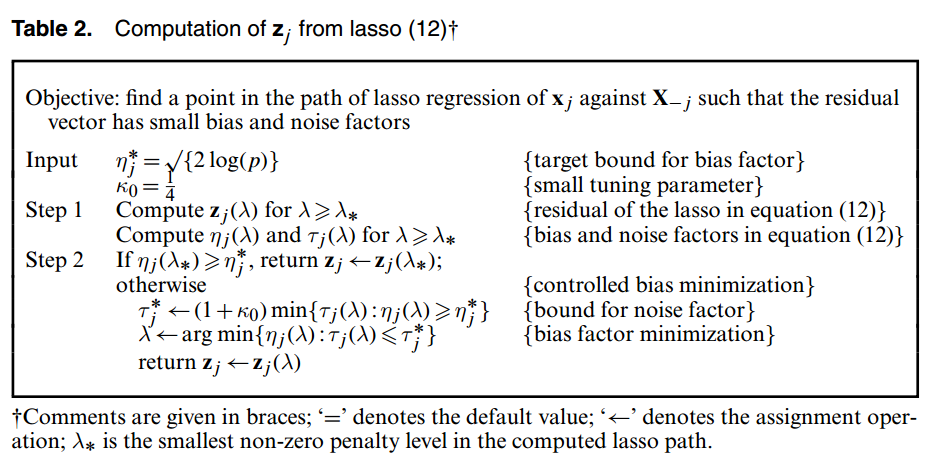
\includegraphics[width=1.0\textwidth]{figs/Table2.png}
  \label{Table2}
\end{figure}
\end{frame}


%----------------------------------------------------------------------------------------
%	PAGE 20
%----------------------------------------------------------------------------------------
%\begin{frame}
%\frametitle{Restricted LDPE}
%\begin{itemize}

%\item[$\blacksquare$] Why use restricted lasso relaxation for $\bz_{j}$?
%  The summands with larger absolute correlation $|\bx_j^T\bx_k/n|$ are likely to have a greater contribution to the bias due to initial estimation error $|\bbeta^{(init)}_k-\beta_k|$.

%\item[$\blacksquare$] How to implement restricted LDPE(RLDPE)?
% Force smaller $|\bz_j^T\bx_k/n|$ for large $|\bx_j^T\bx_k/n|$ with a weighted relaxation:
%\begin{equation}
%\bz_j = \bx_j - \bX_{-j}\gamma_j,\qquad \gamma_j = \argmin_{\bb}{\frac{\|\bx_j-\bX_{-j}\bb\|_2^2}{2n} + \lambda_j\sum_{k\neq j}w_k|b_k|\},
%\end{equation}
%with $w_k$ being a decreasing function of the absolute correlation $|\bx_j^T\bx_k/n|$.
%\item[] Simply set $w_k=0$ for large $|\bx_j^T\bx_k/n|$ and $w_k=1$ for other $k$ in the RLDPE.

%\end{itemize}
%\end{frame}
\begin{frame}
\frametitle{Restricted LDPE}
\begin{itemize}
\item[$\blacksquare$] The reason for using restricted lasso relaxation for $\bz_j$.

  \begin{itemize}
  \item[$\blacktriangleright$]The summands with larger absolute correlation $|\bx_j^T\bx_k/n|$ are likely to have a greater contribution to the bias due to initial estimation error $|\hat{\bbeta}^{(init)}_k-\beta_k|$.
  \end{itemize}
\item[$\blacksquare$] How to implement restricted LDPE(RLDPE)?
  \begin{itemize}
  \item[$\blacktriangleright$] Force smaller $|\bz_j^T\bx_k/n|$ for large $|\bx_j^T\bx_k/n|$ with a weighted relaxation:
  \end{itemize}
  \begin{equation}
  \bz_j = \bx_j - \bX_{-j}\gamma_j,\quad \gamma_j = \mathop{\arg\min}_{\bb}\left\{\frac{\|\bx_j-\bX_{-j}\bb\|_2^2}{2n} + \lambda_j\sum_{k\neq j}w_k|b_k|\right\},
  \end{equation}
%with $w_k$ being a decreasing function of the absolute correlation $|\bx_j^T\bx_k/n|$.

\item[$\blacksquare$] Simply set $w_k=0$ for large $|\bx_j^T\bx_k/n|$ and $w_k=1$ for other $k$ in the RLDPE.

\end{itemize}
\end{frame}


%----------------------------------------------------------------------------------------
%	PAGE 21
%----------------------------------------------------------------------------------------
\begin{frame}
\frametitle{Confidence interval}
\scriptsize
\begin{itemize}
\item[$\blacksquare$] The covariance of the noise component in (\ref{bias(5)}) is proportional to
\begin{equation}
\bV=(V_{jk})_{p\times p},\quad V_{jk} = \frac{\bz_j^T\bz_k}{|\bz_j^T\bx_j||\bz_k^T\bx_k|}
= \sigma^{-2} cov \Big(\frac{\bz_j^T\varepsilon}{\bz_j^T\bx_j}, \frac{\bz_k^T\varepsilon}{\bz_k^T\bx_k}\Big).
\end{equation}

\item[$\blacksquare$]
For sparse vectors $\ba$ with bounded $\|\ba\|_0$,
%e.g. $\|\ba\|_0=2$ for a contrast between two regression coefficients,
an approximate $(1-\alpha)100\%$ confidence interval is
\begin{equation}
\label{LDPE-CI}
\big|\ba \t \hat{\bbeta} - \ba^T\bbeta\big| \le \hat{\sigma}\Phi^{-1}(1-\alpha/2)(\ba^T\bV\ba)^{1/2},
\end{equation}
where $\hat{\bbeta} = (\hat{\beta}_1,\ldots,\hat{\beta}_p) \t$ is the vector of LDPEs $\hat{\beta}_j$ in (\ref{LDPE}), $\Phi$ is the standard normal distribution function.

\end{itemize}
\end{frame}


%----------------------------------------------------------------------------------------
%	PAGE 22
%----------------------------------------------------------------------------------------
\section{Important theoretical results}
\begin{frame}
\sectionpage
\end{frame}

%----------------------------------------------------------------------------------------
%	PAGE 23
%----------------------------------------------------------------------------------------
\begin{frame}
\begin{block}{Proposition 1}
\scriptsize
(a) In the Lasso path, $\|\bz_j(\lambda)\|_2$, $\eta_j(\lambda)$, and $\sigma_j(\lambda)$
are nondecreasing functions of $\lambda$, and $\tau_j(\lambda)\le 1/\|\bz_j(\lambda)\|_2$. Moreover,
$\gamma_j(\lambda)\neq 0$ implies $\eta_j(\lambda)=\lambda n/\|\bz_j(\lambda)\|_2$. \\

(b) Let $\lambda_{univ}=\sqrt{(2/n)\log p}$. Then,
\begin{equation}
\setlength{\abovedisplayskip}{3pt} %%% 3pt 个人觉得稍妥,可自行设置
\setlength{\belowdisplayskip}{3pt}
\sigma_j(C\lambda_{univ})>0 \hbox{ iff } \{\lambda>0: \eta_j(\lambda) \le C\sqrt{2\log p}\}\neq \emptyset,
\end{equation}
    and in this case, the algorithm in Table 2 provides
\begin{gather}
\setlength{\abovedisplayskip}{3pt} %%% 3pt 个人觉得稍妥,可自行设置
\setlength{\belowdisplayskip}{3pt}
\eta_{j}\leq \eta_j^*\le (1\vee C)\sqrt{2\log p},\\
\tau_j\le n^{-1/2}(1+\kappa_0)/\hat{\sigma}_j(C\lambda_{univ}).
\end{gather}
    Moreover, when $\bz_j(0)=\bx_j^\perp =0$, $\eta_j(0+) \inf\{\|\gamma_j\|_1: \bX_{-j}\gamma_j=\bx_j\}=\sqrt{n}$.\\
(c) Let $0<a_0<1\leq C_0<\infty$. Suppose that for $s=a_0n/\log p$
\begin{equation*}
\setlength{\abovedisplayskip}{3pt} %%% 3pt 个人觉得稍妥,可自行设置
\setlength{\belowdisplayskip}{3pt}
\inf_{\delta}\sup_{\bbeta}\Big\{\|\delta(\bX,\by) - \bbeta\|_2^2: \by=\bX\bbeta,
\hbox{$\sum_{j=1}^p$} \min(|\beta_j|/\lambda_{univ},1)\le s+1 \Big\}\le 2C_0s(\log p)/n.
\end{equation*}
\end{block}
\end{frame}


%----------------------------------------------------------------------------------------
%	PAGE 3.1 24
%----------------------------------------------------------------------------------------
\begin{frame}
\begin{block}{Conditions}
\scriptsize
Let $\lambda_{univ}=\sqrt{(2/n)\log p}$. Suppose the model (\ref{LM}) holds with a vector $\bbeta$ satisfying the following capped-$\ell_1$ sparsity condition:
%\vspace{1mm}
\begin{equation}
\label{con19}
\setlength{\abovedisplayskip}{3pt} %%% 3pt 个人觉得稍妥,可自行设置
\setlength{\belowdisplayskip}{3pt}
\sum_{j=1}^p \min\big\{|\beta_j|/(\sigma \lambda_{univ}),1\big\} \leq s.
\end{equation}
This condition holds if $\bbeta$ is $\ell_0$ sparse with $\|\bbeta\|_0 \leq s$ or $\ell_q$ sparse with $\|\bbeta\|_q^q/(\sigma\lambda_{univ})^q \leq s$, $0<q \leq 1$.
Let $\sigma^*=\|\varepsilon\|_2/\sqrt{n}$. A generic condition we impose on the initial estimator is
%\vspace{1mm}
\begin{equation}
\label{con20}
\setlength{\abovedisplayskip}{3pt} %%% 3pt 个人觉得稍妥,可自行设置
\setlength{\belowdisplayskip}{3pt}
P\Big\{ \|\hat{\bbeta}^{(init)} - \bbeta\|_1 \geq C_1 s \sigma^*\sqrt{(2/n)\log(p/\epsilon)}\Big\} \leq \epsilon
\end{equation}
for a certain fixed constant $C_1$ and all $\alpha_0/p^2 \leq \epsilon \leq 1$,
where $\alpha_0\in (0,1)$ is a preassigned constant.
We also impose a similar generic condition on an estimator $\hat{\sigma}$ for the noise level:
%\vspace{1mm}
\begin{equation}
\setlength{\abovedisplayskip}{3pt} %%% 3pt 个人觉得稍妥,可自行设置
\setlength{\belowdisplayskip}{3pt}
\label{con21}
P\Big\{ |\sigma/\sigma^* - 1 | \geq C_2 s (2/n)\log(p/\epsilon) \Big\} \leq \epsilon, \forall \alpha_0/p^2 \leq \epsilon \leq 1,
\end{equation}
with a fixed $C_2$.
%We use the same $\eps$ in (\ref{ell_1-err-bd}) and (\ref{sigma-err-bd}) without much loss of generality.
\end{block}
\end{frame}


%----------------------------------------------------------------------------------------
%	PAGE 3.1 25
%----------------------------------------------------------------------------------------
\begin{frame}%[allowframebreaks]
\begin{block}{Theorem 1}
%\label{th1}
\scriptsize
Let $\hat{\beta}_j$ be the LDPE with an initial estimator $\hat{\bbeta}^{(init)}$.
%Let $\eta_j=\max_{k\neq j}|\bx_k^T\bz_j|/\|\bz_j\|_2$, $\tau_j=\|\bz_j\|_2/|\bx_j^T\bz_j|$,
%$\max(\eps_n',\eps_n'')\to 0$, and $\eta^*>0$.
Let $\eta_j$ and $\tau_j$ be the bias and noise factors in (\ref{defetatau}),
$\sigma^*=\|\varepsilon\|_2/\sqrt{n}$,
$\max(\epsilon_n',\epsilon_n'')\to 0$, and $\eta^*>0$.
Suppose (\ref{con20}) holds with $\eta^*C_1s\sqrt{(2/n)\log(p/\epsilon)} \leq \epsilon_n'$.
If $\eta_j \leq \eta^*$, then
\begin{equation}
\setlength{\abovedisplayskip}{3pt}
\setlength{\belowdisplayskip}{3pt}
\label{thm22}
P\Big\{ \big|\tau_j^{-1}(\hat{\beta}_j - \beta_j) - \bz_j^T \varepsilon/\|\bz_j\|_2\big|
> \sigma^* \epsilon_n'\Big\} \leq \epsilon.
\end{equation}
If in addition (\ref{con21}) holds with $C_2 s (2/n)\log(p/\epsilon)\leq \epsilon_n''$, then for all
$t\ge (1+\epsilon_n')/(1-\epsilon_n'')$,
\begin{equation}
\setlength{\abovedisplayskip}{3pt}
\setlength{\belowdisplayskip}{3pt}
\label{thm23}
P\Big\{|\hat{\beta}_j - \beta_j| \ge \tau_j \hat{\sigma} t \Big\} \leq 2\Phi_{n-1}(-(1-\epsilon_n'')t+\epsilon_n')+2\epsilon,
\end{equation}
where $\Phi_n(t)$ is the student-t distribution function with $n$ degrees of freedom.
Moreover, for the covariance matrix $\bV$ in and all fixed $m$,
\begin{equation}
\setlength{\abovedisplayskip}{3pt} %%% 3pt 个人觉得稍妥,可自行设置
\setlength{\belowdisplayskip}{3pt}
\label{thm24}
\lim_{n\to\infty}
\inf_{\ba\in \mathscr{A}_{n,p,m}}P\Big\{\big|\ba^T\hat{\bbeta} - \ba^T\bbeta\big|
\leq \hat{\sigma}\Phi^{-1}(1-\alpha/2)(\ba^T\bV\ba)^{1/2}\Big\} = 1-\alpha,
\end{equation}
where $\Phi(t) = P\{ N(0,1)\le t\}$ and
$\mathscr{A}_{n,p,m}=\{\ba: \|\ba\|_0 \leq m, \max_{j \leq p}|a_j|\eta_j\leq \eta^*\}$.
\end{block}

\end{frame}


%----------------------------------------------------------------------------------------
%	PAGE 3.3 Remark of theorem 1  26
%----------------------------------------------------------------------------------------
\begin{frame}
\frametitle{Remark 1}
\begin{itemize}
\item[$\blacksquare$] Condition (\ref{thm22}) establishes the joint asymptotic normality of the LDPE under condition (\ref{con20})
    This allows us to write the LDPE as an approximate Gaussian sequence.
\begin{equation}
\setlength{\abovedisplayskip}{3pt}
\setlength{\belowdisplayskip}{3pt}
\label{Gauseq}
\hat{\beta}_j = \beta_j + N(0,\tau_j^2\sigma^2) + o_P(\tau_j\sigma).
\end{equation}

\item[$\blacksquare$] Condition (\ref{thm23}) and (\ref{thm24}) justify the approximate coverage probability of the resulting confidence interval.

\item[$\blacksquare$] The uniform signal strength condition is not required for condition (\ref{con20}) and (\ref{con21}).
\end{itemize}
\end{frame}

%----------------------------------------------------------------------------------------
%	PAGE 3.3
%----------------------------------------------------------------------------------------
%\begin{frame}
%\frametitle{Simultaneous confidence interval}

%\end{frame}

%----------------------------------------------------------------------------------------
%	PAGE 3.3 27
%----------------------------------------------------------------------------------------
\begin{frame}
\frametitle{Simultaneous confidence interval}
\begin{block}{Theorem 2}
%\label{th2}
\scriptsize
Suppose (\ref{con20}) holds with $\eta^*C_1s \sqrt{(2/n)\log(p/\epsilon)} \le \epsilon_n'$. Then,
\begin{equation}
\setlength{\abovedisplayskip}{3pt}
\setlength{\belowdisplayskip}{3pt}
\label{th2-27}
P\Big\{ \max_{\eta_j\le \eta^*} \big|\tau_j^{-1}(\hat{\beta}_j - \beta_j) - \bz_j^T\epsilon/\|\bz_j\|_2\big|
> \sigma^* \epsilon_n'\Big\}\le\epsilon.
\end{equation}
If (\ref{con21}) also holds with $C_2 s (2/n)\log(p/\epsilon)\le \epsilon_n''$, then
\begin{equation}
\setlength{\abovedisplayskip}{3pt}
\setlength{\belowdisplayskip}{3pt}
\label{th2-28}
P\Big\{ \max_{\eta_j\le \eta^*} |\hat{\beta}_j - \beta_j|/(\tau_j\hat{\sigma}) > t\Big\}
\le 2\Phi_n( - (1-\epsilon_n'')t + \epsilon_n')\#\{j:\eta_j\le\eta^*\}+2\epsilon.
\end{equation}
If, in addition to (\ref{con20}) and (\ref{con21}),
$\max_{j\le p}\eta_j\le \eta^*$ and $\max(\epsilon_n',\epsilon)\to 0$ as $\min(n,p)\to \infty$,
then for fixed $\alpha\in (0,1)$ and $c_0>0$,
\begin{equation}
\setlength{\abovedisplayskip}{3pt}
\setlength{\belowdisplayskip}{3pt}
\label{th2-29}
\liminf_{n\to \infty} P\Big\{ \max_{j\le p} \Big|\frac{\hat{\beta}_j - \beta_j}{\tau_j(\hat{\sigma}\wedge \sigma)}\Big|
\le  c_0 + \sqrt{2\log(p/\alpha)}\Big\}  \ge 1-\alpha.
\end{equation}
\end{block}
\end{frame}

%----------------------------------------------------------------------------------------
%	PAGE 3.3 28
%----------------------------------------------------------------------------------------
\begin{frame}
\frametitle{Thresholded LDPE}
\begin{itemize}
\item[$\blacksquare$] From (\ref{th1}), the $\hat{\bbeta}_{j}$ can be viewed as an approximate Gaussian sequence.
\item[$\blacksquare$] The approximate Gaussian sequence is not spare but can be thresholded. Using either the hard or the soft thresholding method:

\begin{equation} \label{TLDPE}
\hat{\bbeta}^{(thr)}_{j}=
\left\{
        \begin{aligned}%{lr}
        & \hat{\bbeta}_{j} I(|\hat{\bbeta}_{j}|>\hat{t}_{j}),   \\
        & sgn(\hat{\bbeta}_{j})(|\hat{\bbeta}_{j}|-\hat{t}_{j})^{+}, \\
        \end{aligned}
\right.
\end{equation}
with
\begin{equation*}
\hat{S}^{(thr)}=\{j:|\hat{\bbeta}_{j}|>\hat{t}_{j}\}
\end{equation*}
where $\hat{t}_j \approx \hat{\sigma}\tau_j\Phi^{-1}(1-\alpha/(2p))$ with $\alpha>0$.
\end{itemize}

\end{frame}


%----------------------------------------------------------------------------------------
%	PAGE $3.3  29
%----------------------------------------------------------------------------------------
\begin{frame}
\begin{block} {Theorem 3}
\scriptsize
    Let $L_0=\Phi^{-1}(1-\alpha/(2p))$, $\tilde{t}_j = \tau_j\sigma L_0$, and
$\hat{t}_j = (1+{c}_n)\sigma\tau_j L_0$ with positive constants $\alpha$ and ${c}_n$. Suppose
condition (queshao) holds with $\eta^*C_1s/\sqrt{n}\leq \epsilon_n'$, $\max_{j\leq p}\eta_j\leq \eta^*$, and
\begin{equation}
P\Big\{\frac{(\hat{\sigma}/\sigma)\vee(\sigma/\hat{\sigma}) -1 + \epsilon_n'\sigma^*/(\hat{\sigma} \wedge \sigma)}
{1-(\hat{\sigma}/\sigma-1)_+ } > {c}_n\Big\} \leq 2\epsilon.
\end{equation}
    Let $\bbeta^{(thr)} = (\beta_1^{(thr)},\ldots,\beta_p^{(thr)})^T$ be the {soft} thresholded LDPE
with these $\hat{t}_j$.
Then, there is an event $\Omega_n$ with $P\{\Omega_n^c\} \leq 3 \epsilon$ such %that
%\begin{equation}
%E\|\bbeta^{( thr)} - \bbeta\|_2^2I_{\Omega_n} \leq \sum_{j=1}^p \min\{\beta_j^2,\tau_j^2\sigma^2(L_0^2(1+2{c}_n)^2+1)\} +(\eps L_n/p)\sigma^2\sum_{j=1}^p\tau_j^2,
%\end{equation}
where $L_n = 4/L_0^3+4{c}_n/L_0+12{c}_n^2L_0$.
Moreover, with at least probability $1-\alpha - 3\epsilon$,
\begin{equation}
\{j: |\beta_j|> (2+2{c}_n)\tilde{t}_j\} \subseteq \hat{S}^{(thr)} \subseteq \{j:\beta_j\neq 0\}.
\end{equation}
\end{block}
\end{frame}


%----------------------------------------------------------------------------------------
%	PAGE $3.3 compare
%----------------------------------------------------------------------------------------
%\begin{frame}
%\frametitle{Thresholded LDPE  VS.  Lasso}
%\begin{itemize}
%\item[$\blacksquare$] Uniform signal strength condition
%\medskip
%\item[$\blacksquare$] Varaible selection
%\medskip
%\item[$\blacksquare$] Thresholded quantities
%\medskip
%\item[$\blacksquare$] $\ell_2$ estimation error
%  \begin{itemize}
%  \item[$\blacktriangleright$] Make no assumption of uniform signal strength condition.
%  \item[$\blacktriangleright$] Large $|\bbeta_{j}|$ are selected by the thresholded LDPE and $\bbeta_{j}=\bzero$ are not select in the presence of small $|\bbeta_{j}|\neq\bzero$.
%  \item[$\blacktriangleright$] Threshold on approximately Gaussian sequence, requires only univariate analysis.
%  \item[$\blacktriangleright$] The order of the $\ell_2$ error bound is slightly sharper than the typical order of $\|\bbeta\|_0\sigma^2\lambda_{univ}^2$ or $\sigma\lambda_{univ}\sum_{j=1}^p \min\big\{|\beta_j|, \sigma\lambda_{univ}\big\}$
%  \end{itemize}

%\bigskip

%\item[$\blacksquare$] Lasso and other regularized methods
%  \begin{itemize}
%  \item[$\blacktriangleright$] Variable selection consistency requires the uniform signal strength condition.
%  \item[$\blacktriangleright$] Can not guaranteed to select correctly variables with large $|\bbeta_{j}|$ or $\bbeta_{j}=\bzero$ in the presence of small $|\bbeta_{j}|\neq\bzero$.
%  \item[$\blacktriangleright$] Thresholded quantities:Thresholding is applied to the gradient $\bX^T(\by-\bX\bbeta)/n$ via the Karush-Kuhn-Tucker-type condition, leading to more complicated nonlinear multivariate analysis.
% \item[$\blacktriangleright$] Rate optimal in the maximum $\ell_2$ estimation loss for many classes of sparse $\bbeta$

%\end{itemize}

%\end{itemize}
%\end{frame}


%----------------------------------------------------------------------------------------
%	PAGE 30
%----------------------------------------------------------------------------------------
\section{Simulation}
\begin{frame}
\sectionpage
\end{frame}


%----------------------------------------------------------------------------------------
%	PAGE 31
%----------------------------------------------------------------------------------------
\begin{frame}
\frametitle{Setting}
Set $n=200$, $p=3000$, and run several simulation experiments with
100 replications in each setting.
\begin{itemize}
\item[$\blacksquare$] Generate independent copy of $(\bX,\by)$: \\
Given a particular $\rho \in(-1,1)$, $\tilde{\bX} = (\tilde{x}_{ij})_{n\times p}$
has iid $N(0,\Sigma)$ rows with $\Sigma = (\rho^{|j-k|})_{p\times p}$,
$\bx_j = \tilde{\bx}_j\sqrt{n}/{|}\tilde{\bx}_j{|}_2$, and $(\bX,\by)$ is as in (\ref{LM}) with $\sigma=1$.
%We also set $\lam_j^*= \lambda_{univ} = \sqrt{(2/n)\log p}$.
% why do we say this here? not used in creating setup.
\item[$\blacksquare$] Generate $\bbeta$: \\
Given a particular $\alpha \geq 1$, $\beta_j = 3\lambda_{univ}$ for $j = 1500, 1800, 2100, \ldots, 3000$,
and $\beta_j = 3\lambda_{univ}/j^\alpha$ for all other $j$, where $\lambda_{univ}=\sqrt{(2/n)\log p}$.
\item[$\blacksquare$] Set $\alpha$ and $\rho$: \\
This simulation example includes four cases, labeled (A), (B), (C), and (D), respectively:
$(\alpha,\rho)=(2,1/5)$, $(1,1/5)$, $(2,4/5)$, and $(1,4/5)$.
\end{itemize}
\end{frame}


%----------------------------------------------------------------------------------------
%	PAGE 32
%----------------------------------------------------------------------------------------
\begin{frame}
\frametitle{Comparison between different methods}
\begin{figure}[h]
  \centering
  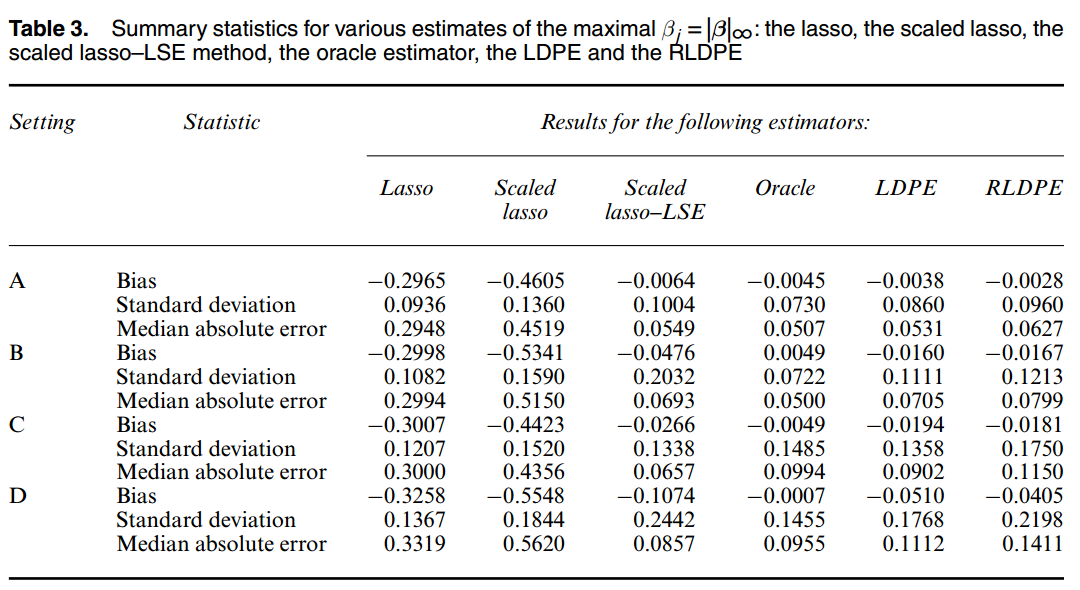
\includegraphics[width=1.0\textwidth]{figs/Table3.png}
  \label{Table1}
\end{figure}
\end{frame}


%----------------------------------------------------------------------------------------
%	PAGE 33
%----------------------------------------------------------------------------------------
\begin{frame}
\frametitle{Histogram of error}
%\begin{figure}[h]
%  \centering
%  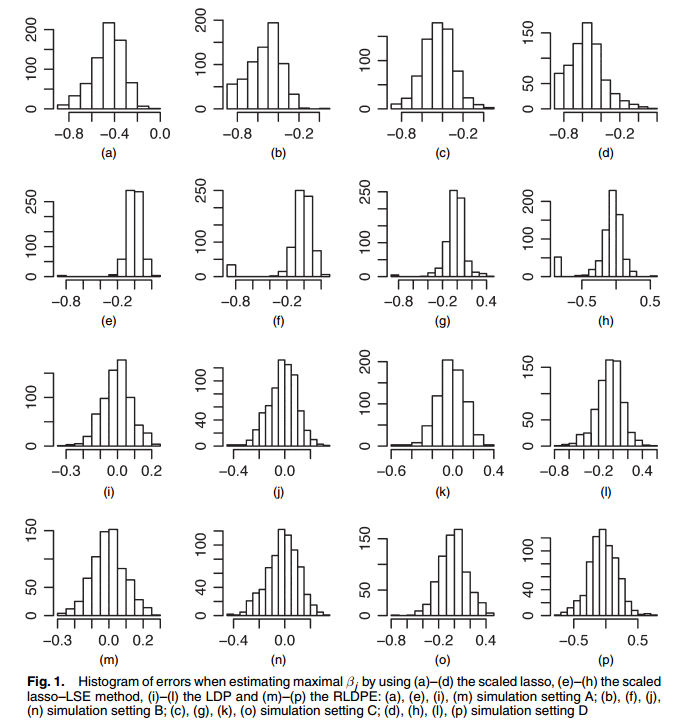
\includegraphics[width=1\textwidth]{figs/Table 4.png}
%  \label{Table4}
%\end{figure}
%\end{frame}

\begin{centering}
\begin{figure}%[ht]
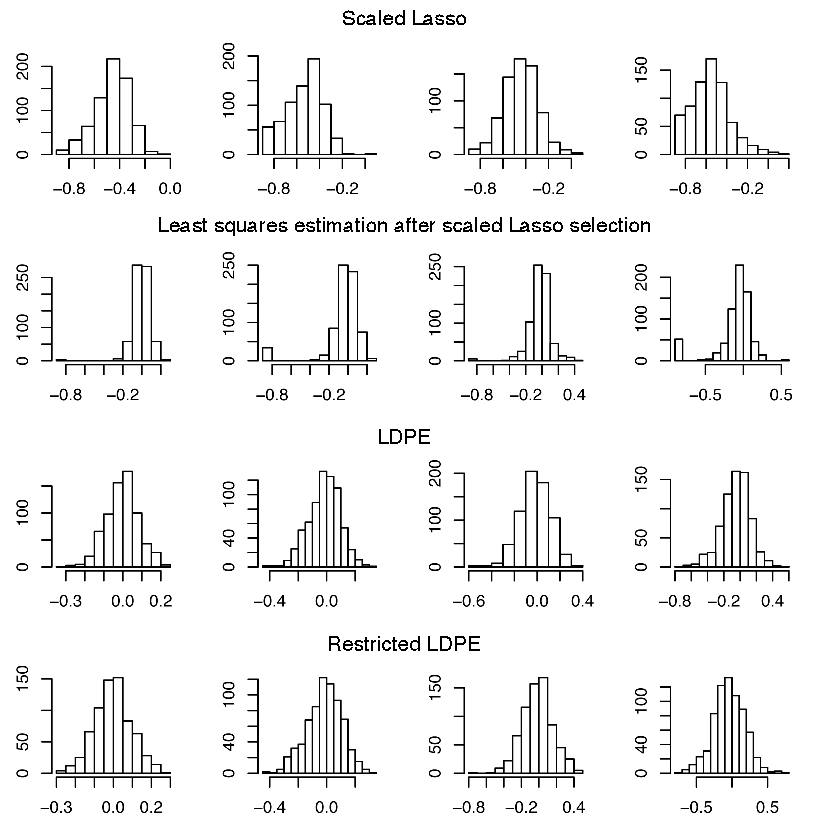
\includegraphics[width = 1.0\textwidth]{1110/hist_diff.pdf}
\caption{Histogram of errors when estimating maximal $\beta_j$ using the scaled Lasso,
{the scaled Lasso-LSE}, the LDPE, and the {R-LDPE}. From left to right,
plots correspond to simulation settings (A), (B), (C), and (D).}
\label{fig:hist}
\end{figure}
\end{centering}

\end{frame}


%----------------------------------------------------------------------------------------
%	PAGE 34
%----------------------------------------------------------------------------------------
\begin{frame}
  \frametitle{Result of mean coverage probability}
  
  \begin{table}[ht]
  \caption{Mean coverage probability of LDPE and R-LDPE.}
  \begin{tabular}{llcccc}
  \toprule
  &&A&B&C&D\\
  \midrule
  all $\beta_j$& LDPE & 0.9597 & 0.9845 & 0.9556 & 0.9855 \\
   &R-LDPE & 0.9595 & 0.9848 & 0.9557 & 0.9885  \\
   maximal $\beta_j$ & LDPE&  0.9571 & 0.9814& 0.9029 &0.9443\\
  & R-LDPE & 0.9614 & 0.9786 & 0.9414 & 0.9786\\
  \bottomrule
  \end{tabular}
  \label{table:meancover}
\end{table}
\end{frame}


%----------------------------------------------------------------------------------------
%	PAGE 35
%----------------------------------------------------------------------------------------
\begin{frame}
\begin{centering}
\begin{figure}%[ht]
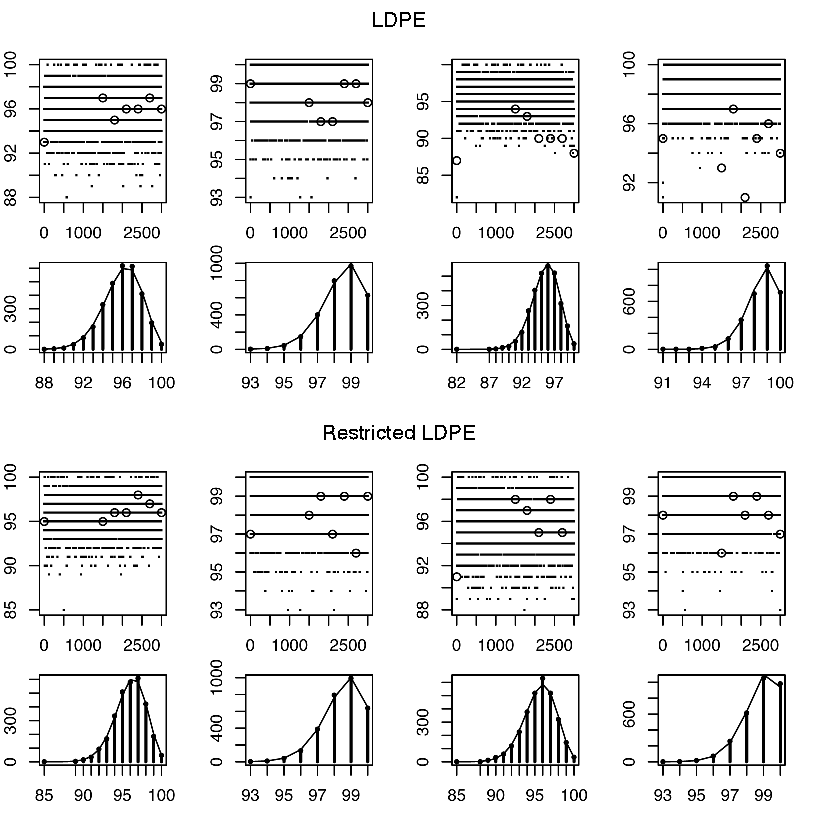
\includegraphics[width = 5cm]{1110/coverage.pdf}
\caption{Rows 1 and 3: Coverage frequencies versus the index of $\beta_j$.
Points corresponding to maximal $\beta_j$ are plotted as large circles.
Rows 2 and 4: The number %percentage
of variables for given values of the relative coverage frequency,
superimposed n the binomial$(100,\tilde p)$ probability mass function,
where $\tilde p$ is the simulated mean coverage.
Figures depict results from simulations A, B, C, and D, from left to right.}
\label{fig:cover}
\end{figure}
\end{centering}

\end{frame}

%----------------------------------------------------------------------------------------
%	PAGE  刘磊的实验结果_1
%----------------------------------------------------------------------------------------
% \begin{frame}
%   \frametitle{Simulation 2———— Mean coverage probability}
%   We set p=300, n=50, replicatiion=100. Generating design matrix $bX$ from different $\Sigma$ to compare the mean coverage probability by LDPE.
%   %\begin{itemize}
%   %\item[$\blacktriangle$] Setting A: $p=300, n=50, replicatiion=100,\Sigma=\rho^{|j-k|}, \rho = 0.2$
%   %\item[$\blacktriangle$] Setting B: $p=300, n=50, replicatiion=100,\Sigma=\rho^{|j-k|}, \rho = 0.8$
%   %\item[$\blacktriangle$] Setting C: $p=300, n=50, replicatiion=100,\Sigma=(\rho)_{300\times300, j\neq k}, \rho = 0.2$
%   %\item[$\blacktriangle$] Setting D:$p=300, n=50, replicatiion=100,\Sigma=(\rho)_{300\times300, j\neq k}, \rho = 0.8$
%   %\end{itemize]
  
%   \begin{table}[ht]
%   \caption{Comparison between different methods.}
%   \begin{tabular}{lcccc}
%   \toprule
%   &&                 &  Lasso  &Scaled lasso  & Scaled lasso-LSE & LDPE \\
%   \midrule
%   Bias               & 2.070   & 2.11         & 2.11             & 0.58 \\
%   Standard deviation & 0.046   & 0.042        & 0.042            & 0.181 \\
%   \bottomrule
%   \end{tabular}
%   \label{liu1}
%   \end{table}
%   \end{frame}


%----------------------------------------------------------------------------------------
%	PAGE  刘磊的实验结果_2
%----------------------------------------------------------------------------------------


%----------------------------------------------------------------------------------------
%	PAGE  刘磊的实验结果_3
%----------------------------------------------------------------------------------------
\begin{frame}
  \frametitle{Simulation 3 -- Mean coverage probability}
  We set p=300, n=50, replicatiion=100. 
  Set 6 non-zero values in $\bbeta$ to compare the mean coverage probability by $\ell_0$ and scaled lasso.
  %Generating design matrix $bX$ from different $\Sigma$ to compare the mean coverage probability by LDPE.
  \begin{itemize}
  \item[$\blacktriangle$] Setting A: $\Sigma=\rho^{|j-k|}, \rho = 0.2$
  \item[$\blacktriangle$] Setting B: $\Sigma=\rho^{|j-k|}, \rho = 0.6$  
  \end{itemize]
  
  % \begin{table}[ht]
  % \caption{Mean coverage probability of $\ell_{0}$ and Scaled lasso.}
  %   \begin{tabular}{llcc}
  %   \toprule
  %   &&                               &   A    &  B   \\
  %   \midrule
  %   all $\beta_j$     & $\ell_{0}$   & 0.915  & 0.942 \\
  %                     & Scaled lasso & 0.907  & 0.953 \\
  %   maximal $\beta_j$ & $\ell_{0}$   & 0.930  & 0.980 \\
  %                     & Scaled lasso & 0.920  & 0.970 \\
  %   \bottomrule
  %   \end{tabular}
  % \label{liu3}
  % \end{table}
\end{frame}
